%!TEX root = main.tex
\section{Decidability results}

We investigate several decidability and asymptotic complexity questions concerning $k$-synchronizability. In this context, we consider finite-state message passing systems, where each process has a bounded number of local states. First, the reduction of checking $k$-synchronizability to a reachability problem under the synchronous semantics in Section~\ref{sec:verif} demonstrates the decidability of the former. 
Then, we give a class of systems for which the problem of checking whether there exists some $k$ such that they are  $k$-synchronizable is decidable.

\begin{theorem}
The problem of checking $k$-synchronizability of a finite-state system $\mathcal{S}$ is decidable and ???-complete.
\end{theorem}
\begin{proof}
Direct consequence of Theorem~\ref{th:main-verif}.
\end{proof}

\begin{figure}
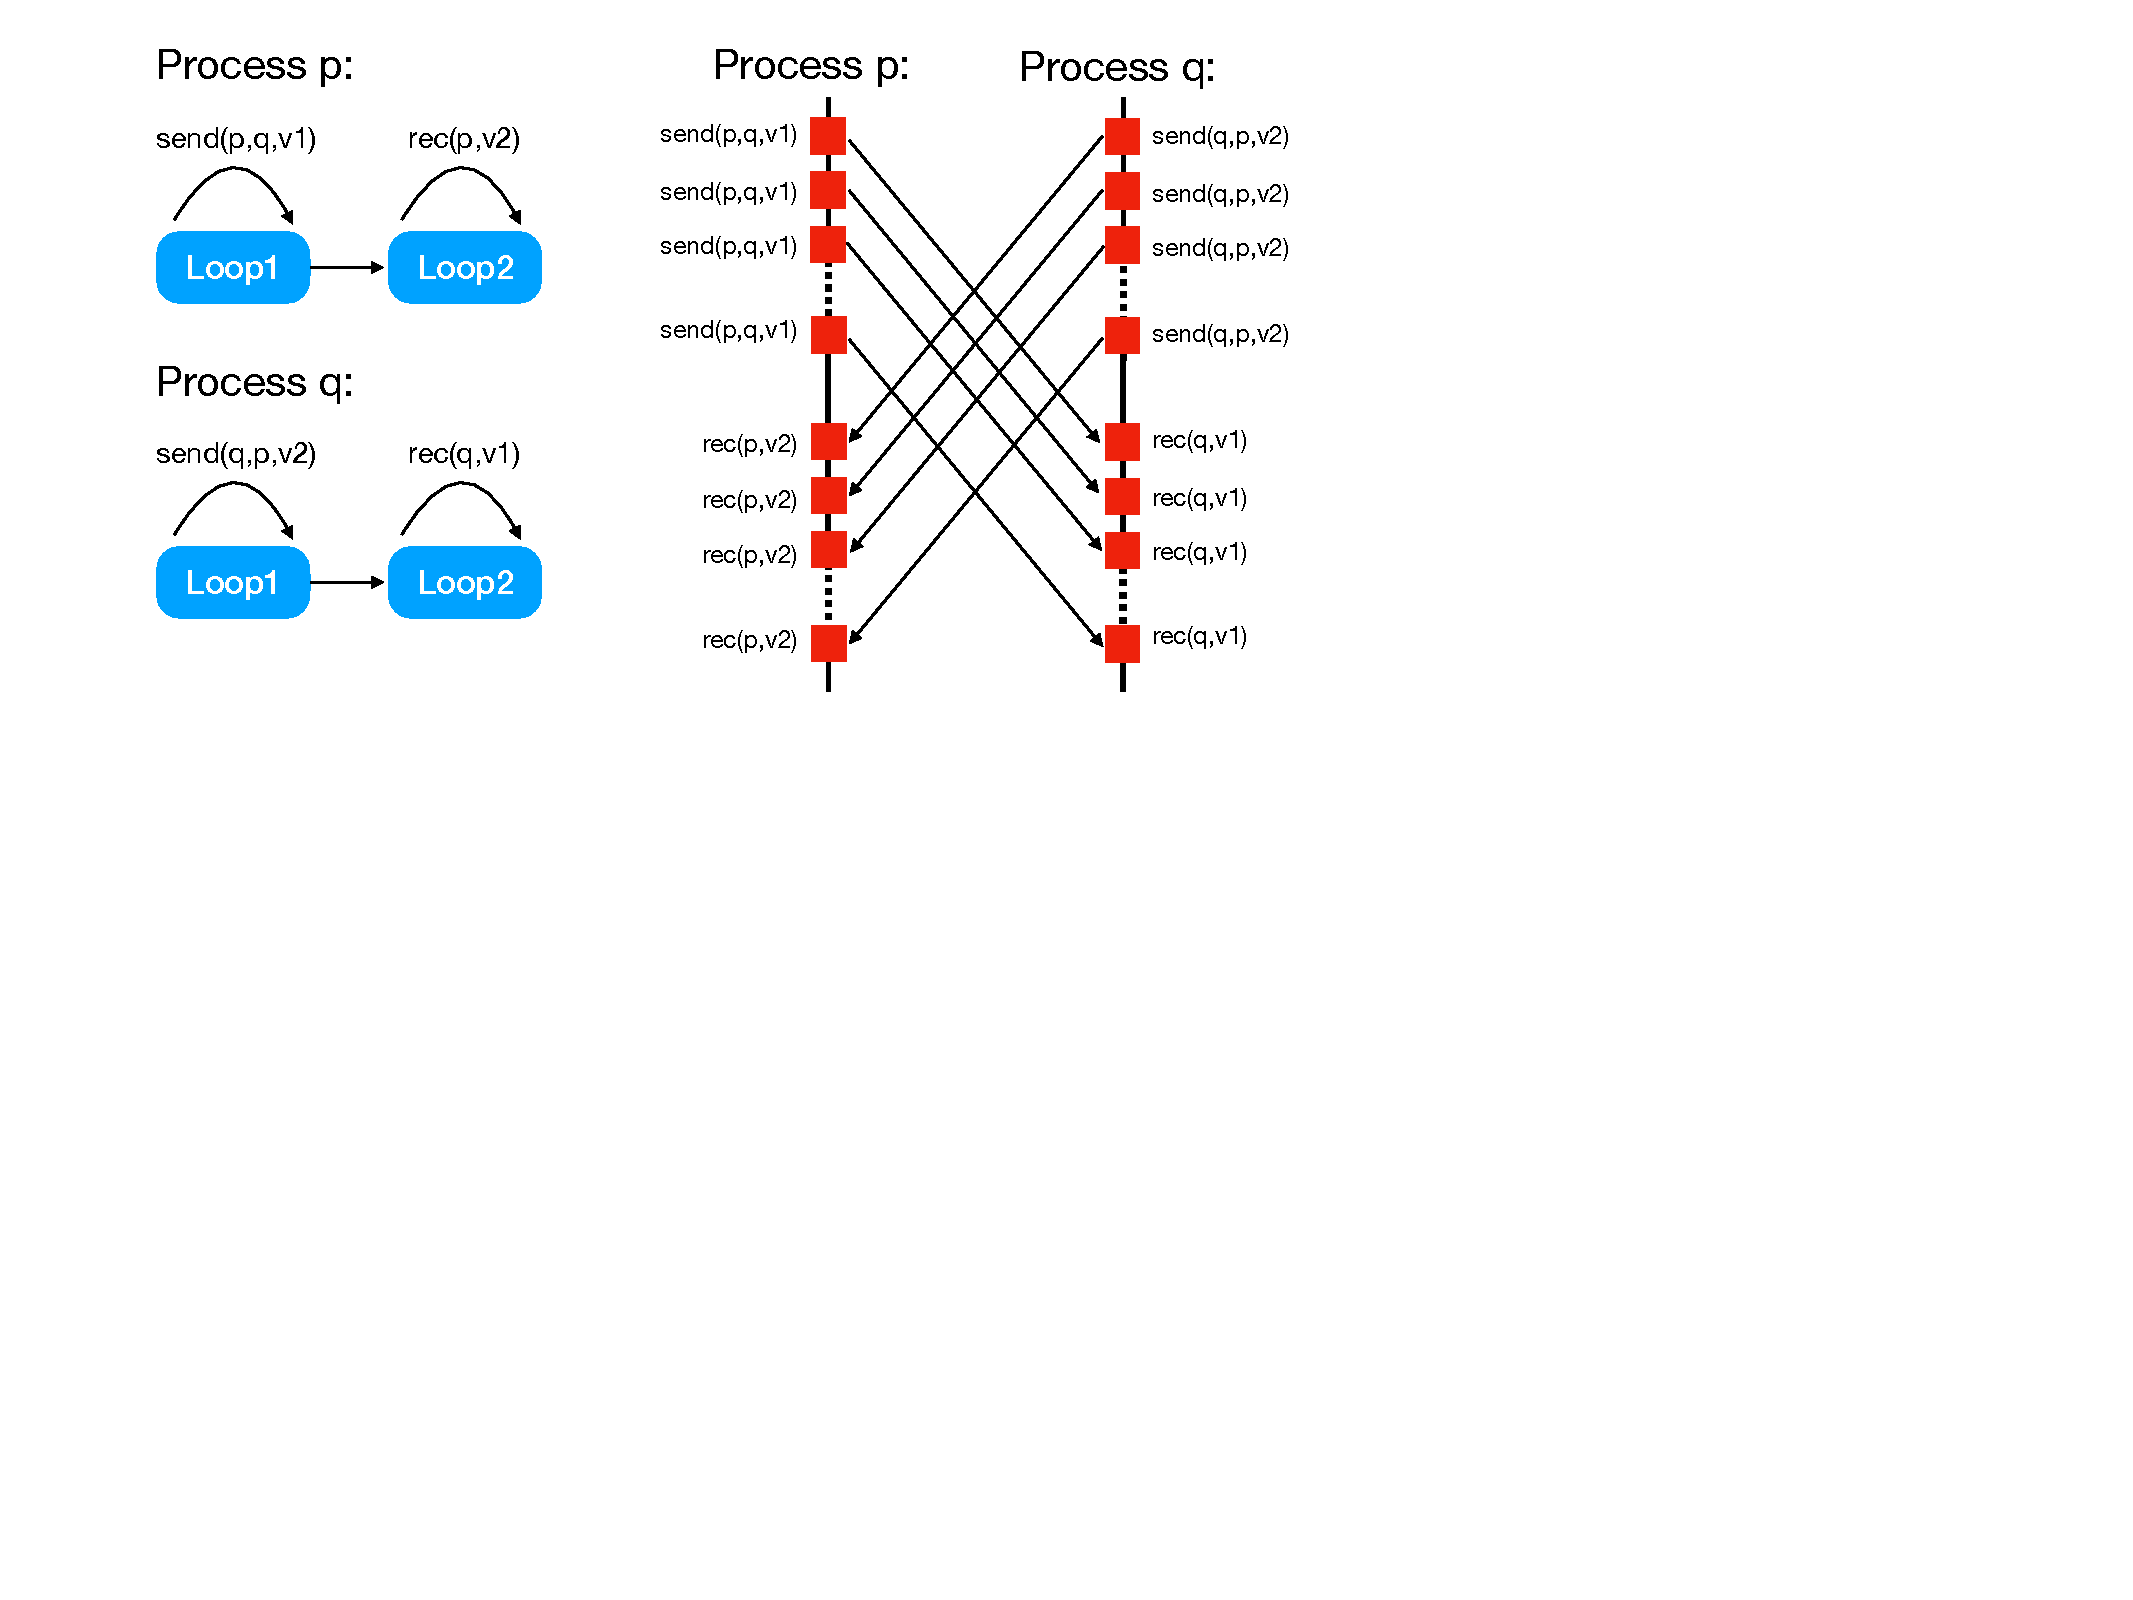
\includegraphics[width=7cm]{Ex-Decidability.pdf}
\caption{An example of a system which is not $k$-synchronizable, for every $k$.}
\label{fig:decid_ex}
\end{figure}

In general, there are two reasons for which a system is not $k$-synchronizable, for every $k$. Either it admits an execution with a bad conflict-graph cycle (e.g., the execution in Figure~\ref{fig:ex-rs-cycle}), or it admits executions with infinitely increasing conflict-graph cycles. Figure~\ref{fig:decid_ex} gives an example of such a system. 
The two loops in each process allow to create executions with unboundedly many send actions before any receive is enabled. However, this example is rather artificial, and up to our knowledge, such scenarios are not present in practical systems. 

Let $\mathcal{S}=((\<Lsts>_p,\delta_p,l_p^0)\mid p\in\<Pids>)$ be a message passing system. A process $p$ is called $k$-bounded when intuitively, it can perform at most $k$ consecutive sends or receives. Formally, for every sequence $w\in (S_{id}\cup R_{id})^*$ accepted by the labeled transition system $(\<Lsts>_p,\delta_p,l_p^0)$, there exists no decomposition $w=w_1\cdot w_2\cdot w_3$ where $w_2\in S_{id}^*\cup R_{id}^*$ and the length of $w_2$ is strictly bigger than $k$. For instance, all the processes in the distributed commit protocol in Figure~\ref{fig:commit} are $2$-bounded (more precisely, the manager is $2$-bounded and the rest of the processes are $1$-bounded). On the other hand, the processes in Figure~\ref{fig:elevator} are not $k$-bounded, for every $k$.